\documentclass[11pt]{article}

\usepackage[utf8]{inputenc}
\usepackage[T1]{fontenc}
\usepackage[margin=1in]{geometry}
\usepackage{amsmath,amssymb}
\usepackage{booktabs}
\usepackage{longtable}
\usepackage{graphicx}
\usepackage{xcolor}
\usepackage{enumitem}
\usepackage{natbib}
\usepackage[hidelinks]{hyperref}

\title{\textbf{Complexity-Graded Head Recruitment:\\
Dead Attention Heads as a Behavioural Probe of Task Demand\\
in Transformer Language Models}}
\author{(author list omitted in draft)}
\date{\today}

\newcommand{\dl}{d(\ell)}

\begin{document}
\maketitle

\begin{abstract}
A transformer attention head is \emph{dead} for a given prediction when its
attribution score falls below a fixed fraction of the strongest head in its
layer: the head sits on the residual stream but routes essentially no
information for that input. We treat the per-layer count of dead heads,
$\dl$, as a first-class observable and ask how it deforms as a task becomes
more demanding. Measuring six models (GPT-2 medium/large/xl; Pythia
70M/160M/410M) across two controlled task ladders---an eight-step
complexity gradient and a clean six-step serial-reasoning ladder
(1-hop$\,\ldots\,$6-hop chains with surface form held fixed)---we find one
robust phenomenon: \textbf{as task demand rises, models monotonically
recruit dead heads into active computation.} The recruitment is large and
universal at the first reasoning step (the 1-hop$\to$2-hop transition
activates $20$--$55\%$ of all previously dead heads in every model), and the
size of the recruitable reserve scales with model capacity (GPT-2~xl idles
$19\%$ of its heads on the easiest chain and draws down $11$ percentage
points of that across the ladder, versus $8\%/3.7$\,pp for GPT-2~medium and
$6\%/2.1$\,pp for Pythia-70M). The recruitment is, moreover, \emph{spatially
directed}: as reasoning depth rises the dead zone's front edge retreats
deeper and early layers are drawn into computation---the network's
\emph{active frontier} extends. The two deformations are coupled and both
strengthen with scale (Llama-3-8B reasoning subset: $r(\text{hops},
\text{total dead}){=}{-}0.89$ \emph{and} $r(\text{hops}, \text{frontier
depth}){=}{+}0.96$; pooled frontier correlation $r{=}{+}0.70$ over the three
largest GPT-2/Pythia models). We thus describe a two-axis demand--geometry
law: rising demand both \emph{deflates} the dead-head landscape (vertical
recruitment) and \emph{advances} its active frontier (horizontal extension),
at an estimable cost of $\sim$1--2 layers per reasoning hop in the cleanest
model. A controlled $(D,W)$ factorial that varies serial depth and parallel
width independently confirms the width half of the mechanism on Llama-3-70B
(parallel width recruits heads, $r{=}{+}0.81$; serial depth does not), while
showing the depth half needs smaller, lower-reserve models to resolve. We
report the complete per-model, per-task dataset (84 measurements) and lay out
the experiments needed to turn these observations into a publishable result.
\end{abstract}

% ======================================================================
\section{Introduction}
% ======================================================================
Residual transformers expose, at every layer, two routes for information: a
\emph{compute path} through the attention heads and the feed-forward (FFN)
block, and an \emph{identity residual path} that bypasses them. A large
body of work establishes that the compute path is heavily underused---most
attention heads can be pruned with little loss
\citep{michel2019sixteen,voita2019analyzing}, deep layers are frequently
redundant \citep{men2024shortgpt,gromov2024unreasonable}, and harder inputs
deserve more computation \citep{graves2016adaptive,schuster2022confident}.
What is missing is a \emph{graded, per-task} account: not ``which heads are
removable in general,'' but \textbf{how the set of working heads grows as a
task becomes harder, and how that growth is bounded by model capacity.}

We make the dead-head landscape $\dl$---the number of attention heads at
layer $\ell$ whose attribution falls below an activity threshold---a
first-class measurement, and track how it changes along a controlled
complexity axis. Our central finding is a single, directional law:

\begin{quote}
\emph{The dead-head landscape deflates monotonically as task demand rises:
the model recruits dormant heads to pay for additional computation. The
recruitable reserve, and how much of it is drawn down, scale with model
size.}
\end{quote}

We deliberately restrict this paper to the recruitment phenomenon and its
scaling. We \emph{do not} make claims about output entropy or about a
saturation/exit depth; those analyses are out of scope here and are left to
companion work.

\paragraph{Contributions.}
\begin{enumerate}[leftmargin=1.4em,itemsep=2pt]
\item We define and measure the dead-head landscape $\dl$ as a graded
function of task demand across six models and two task ladders
(Section~\ref{sec:method}).
\item We establish \emph{complexity-graded head recruitment} (the vertical
axis): dead-head count falls monotonically with reasoning depth, with a
universal step-change at the first reasoning hop (Section~\ref{sec:recruit}).
\item We show the recruitable reserve \emph{dilates with model scale}
(Section~\ref{sec:scale}).
\item We establish the \emph{horizontal axis}: recruitment is spatially
directed---the active frontier extends deeper as reasoning depth rises, at a
measurable per-hop layer cost, giving a coupled two-axis demand--geometry law
(Section~\ref{sec:frontier}).
\item We release the complete 84-measurement dataset (Appendix~\ref{app:data})
and a precise experimental roadmap (Section~\ref{sec:roadmap}).
\end{enumerate}

% ======================================================================
\section{Related work}
% ======================================================================
\paragraph{Attention-head and layer redundancy.}
\citet{michel2019sixteen} showed that a large fraction of attention heads can
be pruned at test time with negligible loss, and that importance is highly
uneven across heads. \citet{voita2019analyzing} reached a similar conclusion
for encoder self-attention, identifying a small set of specialised heads
(positional, syntactic, rare-token) that do most of the work while the rest
are removable. At the layer level, \citet{men2024shortgpt} introduce a
\emph{Block Influence} score---the degree to which a block changes the hidden
state---and find many deep layers contribute little; \citet{gromov2024unreasonable}
likewise prune large contiguous spans of late layers with small degradation.
\citet{fan2020reducing} (LayerDrop) and \citet{sajjad2023effect} study
structured layer dropping during and after training. \emph{All of this work
treats redundancy as a (largely) static property of a trained network. Our
contribution is to make redundancy a measured, monotone function of task
demand---the dead set is not fixed but is drawn down as the task gets
harder.}

\paragraph{Conditional and adaptive computation.}
\citet{graves2016adaptive} introduced Adaptive Computation Time, letting a
recurrent model learn how many steps to spend per input. The idea was carried
into transformers by Universal Transformers \citep{dehghani2019universal} and
by depth-adaptive / early-exit methods
\citep{elbayad2020depth,xin2020deebert,schuster2022confident}, which halt
computation once a per-token confidence criterion is met.
\citet{raposo2024mixture} (Mixture-of-Depths) route only some tokens through
each block. \emph{These methods adapt essentially one scalar---how deep to
go. We provide evidence for a second, orthogonal axis the model already uses
internally: how \emph{wide} (how many heads) to engage at each layer, as a
graded function of demand.}

\paragraph{Reasoning, multi-hop recall, and serial computation.}
A complementary line studies where multi-step computations occur.
\citet{geva2023dissecting} and \citet{meng2022locating} localise factual
recall to specific layers and modules; \citet{yang2024large} show that
multi-hop reasoning is performed latently across successive layer ranges, and
\citet{biran2024hopping} show that later hops in a chain resolve in later
layers and can fail when there is insufficient depth. On the theoretical
side, \citet{merrill2023parallelism} characterise the limited parallel
complexity class of fixed-depth transformers, and subsequent work
\citep{feng2023towards,li2024chain} shows that chain-of-thought effectively
adds serial computation steps. \emph{These works motivate using a
serial-reasoning ladder as a clean complexity axis; we measure how the
internal active-head set responds to it.}

\paragraph{Stages of inference and residual-stream analysis.}
\citet{lad2024remarkable} argue that inference proceeds through a small number
of qualitatively distinct stages (detokenisation, feature construction,
prediction, sharpening), which is consistent with the conserved structure we
observe (Section~\ref{sec:skeleton}). The logit lens
\citep{nostalgebraist2020logitlens} and tuned lens
\citep{belrose2023eliciting} read out the \emph{content} of the residual
stream by depth. \emph{We instead study the \emph{routing}: which compute
units carry attribution, and how their number changes with task demand.}

\paragraph{Circuits and attribution.}
Mechanistic circuit work names specific components for specific tasks: a
mathematical framework for the residual stream \citep{elhage2021mathematical},
the indirect-object-identification circuit \citep{wang2022interpretability},
and automated circuit discovery \citep{conmy2023towards} built on attribution
patching \citep{nanda2023attribution}; \citet{ferrando2024information} trace
information-flow routes at scale. \emph{We use the same per-head attribution
criterion, but study the aggregate complement---the dead set---across a graded
task family, a level of description above any single circuit.}

% ======================================================================
\section{Method}\label{sec:method}
% ======================================================================
\paragraph{Dead heads.}
For a prompt $p$ we compute, for each attention head $(\ell,h)$, a scalar
attribution score $s(\ell,h)$ via gradient$\,\times\,$activation on the head's
output (the per-head attribution of \texttt{compute\_per\_head\_scores} in the
analysis pipeline). A head is \emph{dead} for $p$ iff
\[
s(\ell,h) \;<\; \tau \cdot \max_{h'} s(\ell,h'), \qquad \tau = 0.15,
\]
i.e.\ it carries less than $15\%$ of the attribution of the strongest head in
its own layer. The \emph{dead-head landscape} is
$\dl = \#\{\,h : (\ell,h)\text{ dead}\,\}$, and the total dead count is
$\sum_\ell \dl$.

\paragraph{Models.}
Six pretrained models spanning two families and a range of depth/width:
GPT-2 medium ($24\text{L}\times16\text{H}$), large ($36\times20$), xl
($48\times25$); Pythia-70M ($6\times8$), 160M ($12\times12$), 410M
($24\times16$).

\paragraph{Task ladders.}
\begin{itemize}[leftmargin=1.4em,itemsep=2pt]
\item \textbf{deep\_chains} --- a \emph{pure serial-reasoning ladder}:
``\texttt{A is the parent of B. B is the parent of C.\ \ldots\ A's $k$-th
descendant is}'' for $k=1\ldots6$. Each rung adds exactly one composition
step; the surface template is held fixed, isolating reasoning depth.
\item \textbf{complexity\_gradient} --- eight heterogeneous tasks ordered by
nominal difficulty: lexical, subject--verb agreement, 1-hop factual,
arithmetic, 2-hop, 3-hop, syllogism, analogy. Its 1/2/3-hop reasoning subset
is a secondary controlled axis.
\end{itemize}

\paragraph{Measurements.}
For every (model, task) chart we report total dead heads; the dead fraction
$\sum_\ell\dl / (L\cdot H)$; the dead-mass \emph{centroid} in fractional depth
($0=$ first layer, $1=$ last); the fraction of dead mass in the front half of
the network; and the \emph{front-edge depth} $q_{25}$---the normalised depth
at which the first quarter of dead mass accumulates. $q_{25}$ is our primary
horizontal-axis statistic because, unlike the centroid, it is not dominated by
the task-invariant sparse readout region at the back of the network and so is
sensitive to where the \emph{active frontier} sits. The complete set of
$6\times8 + 6\times6 = 84$ measurements is listed in Appendix~\ref{app:data}.

\paragraph{Auxiliary exact data.}
To corroborate the figure-recovered trends with ground-truth attribution we
additionally analyse one model, Llama-3-8B ($32\text{L}\times32\text{H}$), for
which exact per-head dead masks are available from the analysis pipeline (read
directly from the per-head graph files, not recovered from a rendered chart).
We use it only as a high-fidelity check on the two-axis correlations.

\paragraph{Data provenance and recovery.}
The sweep was archived as rendered per-layer bar charts (the
\texttt{abdulla\_results/} directory; subfolders \texttt{graphs},
\texttt{graphs~2}, \texttt{graphs~3}). Because the underlying numeric arrays
were not saved, we recover per-layer counts directly from the images with a
calibrated extractor (\texttt{extract\_dead\_heads.py}): the $y$-axis is
calibrated from the rendered ``total heads $=N$'' line and the plot baseline,
and each layer's bar height is read as a contiguous run anchored at the
baseline. Recovered values were validated against the printed bar labels on
GPT-2~xl and GPT-2~large to within $\pm1$--$2$ heads. We treat the recovered
data as reliable for trend analysis; regenerating exact arrays from the
pipeline is the first item on the roadmap (Section~\ref{sec:roadmap}).

% ======================================================================
\section{Results}
% ======================================================================

\subsection{Complexity-graded head recruitment}\label{sec:recruit}
Table~\ref{tab:dc-total} reports total dead heads on the serial-reasoning
ladder. Across the larger models the count falls as reasoning depth rises:
the model engages more heads to perform more composition steps. The effect is
strongest and most monotone in the deepest/widest models (GPT-2~xl decreases
on four of five rungs, a net $-131$ heads from 1-hop to 6-hop; Pythia-410M a
net $-24$).

\begin{table}[h]
\centering
\caption{Total dead attention heads on the \texttt{deep\_chains} serial-reasoning
ladder. Fewer dead heads $=$ more heads recruited into active computation.}
\label{tab:dc-total}
\small
\begin{tabular}{lrrrrrr}
\toprule
Model & 1-hop & 2-hop & 3-hop & 4-hop & 5-hop & 6-hop \\
\midrule
GPT-2 medium & 29 & 15 & 11 & 9 & 15 & 15 \\
GPT-2 large & 70 & 34 & 45 & 38 & 47 & 48 \\
GPT-2 xl & 228 & 142 & 115 & 105 & 113 & 97 \\
Pythia-70M & 3 & 2 & 1 & 1 & 4 & 2 \\
Pythia-160M & 22 & 10 & 11 & 16 & 23 & 18 \\
Pythia-410M & 66 & 53 & 56 & 47 & 46 & 42 \\
\bottomrule
\end{tabular}
\end{table}

\paragraph{A universal first-hop cliff.}
The single largest recruitment event is the \mbox{1-hop$\to$2-hop} step---the
introduction of the first genuine composition. It recruits a large fraction of
all idle heads in \emph{every} model:
\begin{center}
\small
\begin{tabular}{lrlr}
\toprule
Model & 1$\to$2 recruited & Model & 1$\to$2 recruited \\
\midrule
GPT-2 medium & $+48\%$ & Pythia-70M  & $+33\%$ \\
GPT-2 large  & $+51\%$ & Pythia-160M & $+55\%$ \\
GPT-2 xl     & $+38\%$ & Pythia-410M & $+20\%$ \\
\bottomrule
\end{tabular}
\end{center}
The same ordering appears in the heterogeneous complexity gradient
(Table~\ref{tab:cg-total}): the surface/lexical, single-hop-factual, and
analogy tasks leave the most heads dead, while the multi-step 2-hop and 3-hop
reasoning tasks engage the most heads (e.g.\ GPT-2~xl: lexical $311$ vs.\
2-hop $142$, 3-hop $115$).

\begin{table}[h]
\centering
\caption{Total dead heads on the \texttt{complexity\_gradient} suite. Easy
surface tasks leave the most heads dead; multi-step reasoning engages the most.}
\label{tab:cg-total}
\scriptsize
\begin{tabular}{lrrrrrrrr}
\toprule
Model & Lexical & Subj-verb & 1-hop fact & Arithmetic & 2-hop & 3-hop & Syllogism & Analogy \\
\midrule
GPT-2 medium & 60 & 37 & 57 & 38 & 15 & 11 & 35 & 38 \\
GPT-2 large & 106 & 71 & 113 & 94 & 34 & 45 & 101 & 120 \\
GPT-2 xl & 311 & 229 & 252 & 212 & 142 & 115 & 228 & 289 \\
Pythia-70M & 7 & 4 & 4 & 4 & 2 & 1 & 3 & 2 \\
Pythia-160M & 31 & 20 & 22 & 21 & 10 & 11 & 17 & 14 \\
Pythia-410M & 69 & 71 & 64 & 45 & 53 & 56 & 69 & 75 \\
\bottomrule
\end{tabular}
\end{table}

\subsection{The recruitable reserve dilates with scale}\label{sec:scale}
Table~\ref{tab:dc-frac} expresses the same data as a fraction of all heads.
Two scale effects are visible. First, larger models carry a larger idle
reserve on the easiest task (GPT-2: $8\%\to10\%\to19\%$ for
medium$\to$large$\to$xl at 1-hop). Second, they exercise a wider dynamic
range across the ladder (drawing down $3.7$, $3.1$, and $10.9$ percentage
points respectively). The model behaves as though capacity is a reserve held
against demand: the more capacity, the more is held idle when it is not
needed, and the more can be mobilised when it is.

\begin{table}[h]
\centering
\caption{Dead heads as a fraction of all heads on \texttt{deep\_chains}.}
\label{tab:dc-frac}
\small
\begin{tabular}{lrrrrrr}
\toprule
Model & 1-hop & 2-hop & 3-hop & 4-hop & 5-hop & 6-hop \\
\midrule
GPT-2 medium & 8\% & 4\% & 3\% & 2\% & 4\% & 4\% \\
GPT-2 large & 10\% & 5\% & 6\% & 5\% & 7\% & 7\% \\
GPT-2 xl & 19\% & 12\% & 10\% & 9\% & 9\% & 8\% \\
Pythia-70M & 6\% & 4\% & 2\% & 2\% & 8\% & 4\% \\
Pythia-160M & 15\% & 7\% & 8\% & 11\% & 16\% & 12\% \\
Pythia-410M & 17\% & 14\% & 14\% & 12\% & 12\% & 11\% \\
\bottomrule
\end{tabular}
\end{table}

\subsection{The horizontal axis: the active frontier extends with
demand}\label{sec:frontier}
Recruitment has not only a magnitude but a \emph{direction}. We ask where in
depth the recruited heads come from by tracking the front edge of the
dead-head distribution---the normalised depth $q_{25}$ at which the first
quarter of dead mass has accumulated (a front-sensitive statistic, unlike the
centroid, which is anchored by the task-invariant sparse readout region at the
back). As reasoning depth rises, $q_{25}$ moves deeper: the dead zone retreats
and the \emph{active frontier} advances. Table~\ref{tab:twoaxis} reports both
axes together as correlations with hop count.

\begin{table}[h]
\centering
\caption{The two coupled axes on \texttt{deep\_chains}, plus the exact
Llama-3-8B reasoning subset (1/2/3-hop, per-head attribution, not
figure-recovered). Negative $r(\text{hops},\text{total})$ is recruitment
(vertical axis); positive $r(\text{hops},q_{25})$ and
$r(\text{hops},\text{centroid})$ is frontier extension (horizontal axis).
Both effects appear in the deep/wide models and strengthen with scale; the
smallest models saturate.}
\label{tab:twoaxis}
\small
\begin{tabular}{llrrr}
\toprule
Model & Geom (L$\times$H) & $r$(hops, total) & $r$(hops, $q_{25}$) & $r$(hops, centroid) \\
\midrule
GPT-2 xl & 48$\times$25 & $-0.82$ & $+0.48$ & $+0.78$ \\
GPT-2 large & 36$\times$20 & $-0.33$ & $+0.88$ & $+0.29$ \\
Pythia-410M & 24$\times$16 & $-0.93$ & $+0.72$ & $+0.66$ \\
GPT-2 medium & 24$\times$16 & $-0.55$ & $-0.34$ & $-0.32$ \\
Pythia-160M & 12$\times$12 & $+0.24$ & $-0.61$ & $-0.59$ \\
Pythia-70M & 6$\times$8 & $+0.05$ & $-0.65$ & $-0.65$ \\
\midrule
\textbf{Llama-3-8B} & 32$\times$32 & $\mathbf{-0.89}$ & $\mathbf{+0.96}$ & $\mathbf{+1.00}$ \\
\bottomrule
\end{tabular}
\end{table}

The signal is clearest in the model with exact (non-recovered) attribution.
On Llama-3-8B the three-rung reasoning ladder shows total dead falling
($425\to256\to248$), early-layer ($\ell\!\le\!10$) dead falling sharply
($92\to47\to42$), and the frontier advancing monotonically
($q_{25}: 0.46\to0.54\to0.58$; centroid $0.67\to0.71\to0.76$). Among the
figure-recovered models the same coupling holds for the three largest
(GPT-2~xl/large, Pythia-410M): $r(\text{hops},q_{25})$ pools to $+0.70$
($n{=}18$). The three smallest models do not show it---their counts are
quantisation-noisy and, with only $6$--$24$ layers, they appear to exhaust
their reserve within one or two hops, so neither axis has room to move. This
is the same scale dependence seen for recruitment (Section~\ref{sec:scale}):
both axes require spare capacity to be visible.

\paragraph{A per-hop depth cost.}
Converting the frontier shift to absolute layers gives a serial cost per
reasoning step: $\approx1.9$ layers/hop on Llama-3-8B (1$\to$3 hop), and
$0.3$--$0.5$ layers/hop on the larger GPT-2/Pythia chains. The smaller
per-hop cost on the GPT-2 chains is consistent with early saturation---the
frontier stops advancing once the model can no longer carry out additional
hops---which predicts that the frontier should track task \emph{accuracy}, a
test we make explicit in the roadmap (Section~\ref{sec:roadmap}). This
per-hop layer cost is the empirical, per-layer counterpart of the theoretical
result that transformer depth bounds serial computation
\citep{merrill2023parallelism,li2024chain} and the finding that later hops
resolve in later layers and fail without sufficient depth
\citep{yang2024large,biran2024hopping}.

\subsection{A conserved backbone}\label{sec:skeleton}
The recruitment that does occur is a deformation of a stable structure, not a
redrawing of it. Most dead mass sits in the back half of the network at every
difficulty level (front-half fractions are small and roughly constant; see
Appendix~\ref{app:data}): the late layers keep attention sparse regardless of
task, while recruitment is concentrated in the early-to-middle band. This
conserved-then-deformed picture is consistent with the view that inference
proceeds through a small set of qualitatively distinct stages
\citep{lad2024remarkable}.

\subsection{Controlled dissociation: a $(D,W)$ factorial}\label{sec:factorial}
The complexity gradient and deep chains confound \emph{what} kind of demand
rises with \emph{how much}. To test the sharper hypothesis---that
\emph{serial} demand (dependency depth $D$) recruits network \emph{depth}
while \emph{parallel} demand (independent width $W$) recruits attention
\emph{heads} (Figure~\ref{fig:schematic})---we built a factorial task suite
that varies $D$ and $W$ independently: a pure-serial ladder (a constant-length
pointer-chase, $D{=}1\ldots6$, $W{=}1$), a pure-parallel ladder (find a unique
binding among $W$ items, $D{=}1$, $W{=}1\ldots6$, with a length-matched
variant), and a crossed $3{\times}3$ grid. We measure, per task, the recruited
\emph{width} $\hat W$ (active heads per layer) and recruited \emph{depth}
$\hat D$ (the active-frontier depth, i.e.\ the layer quantiles of the
dead-mass distribution). Results are on Llama-3-70B\footnote{Meta-Llama-3-70B,
loaded in bfloat16 with CPU offload; forward-only magnitude metric.} and should
be read as a proof-of-method: the effects are small because, as
Section~\ref{sec:scale} shows, a 70B holds an enormous idle reserve that
compresses all recruitment.

\begin{figure}[t]
\centering
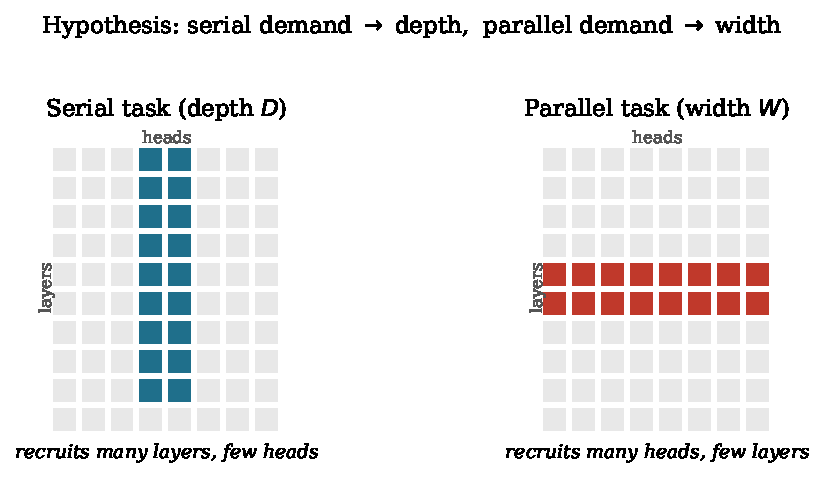
\includegraphics[width=0.86\linewidth]{figs/fig_schematic.pdf}
\caption{The hypothesis. A serial task should recruit a deep, narrow band of
units (many layers, few heads); a parallel task a shallow, wide band (many
heads, few layers). The active subgraph is the task's computation graph
embedded into the layer$\times$head lattice.}
\label{fig:schematic}
\end{figure}

\paragraph{Width recruits heads; depth does not.}
On the length-matched parallel ladder, active heads per layer rise with $W$
($r{=}{+}0.81$; Figure~\ref{fig:axes} left), while the active frontier does not
move ($r(W, q_{25}){=}{-}0.09$). The crossed grid confirms and separates the
two axes: fitting active-heads-per-layer gives
$\approx 32.3 - 0.14\,D + 0.25\,W$---a clean positive width coefficient and a
near-zero depth coefficient (Figure~\ref{fig:grid})---while the depth
coefficient on the frontier is $\approx 0.0005$ (in depth fraction), i.e.\
zero. \textbf{Parallel width engages more heads at fixed depth; serial depth
does not engage more heads.} This is the width half of the predicted double
dissociation.

\begin{figure}[t]
\centering
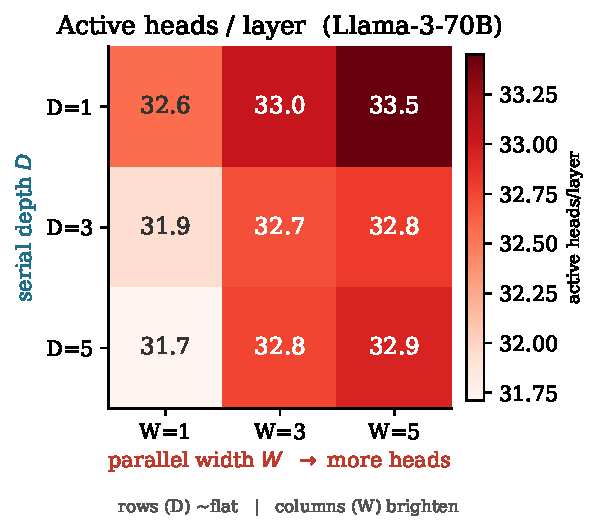
\includegraphics[width=0.66\linewidth]{figs/fig_grid.pdf}
\caption{Active heads per layer across the crossed $(D,W)$ grid on
Llama-3-70B. Columns brighten with parallel width $W$ (more heads engaged);
rows are flat across serial depth $D$. Fit: $32.3-0.14\,D+0.25\,W$.}
\label{fig:grid}
\end{figure}

\begin{figure}[t]
\centering
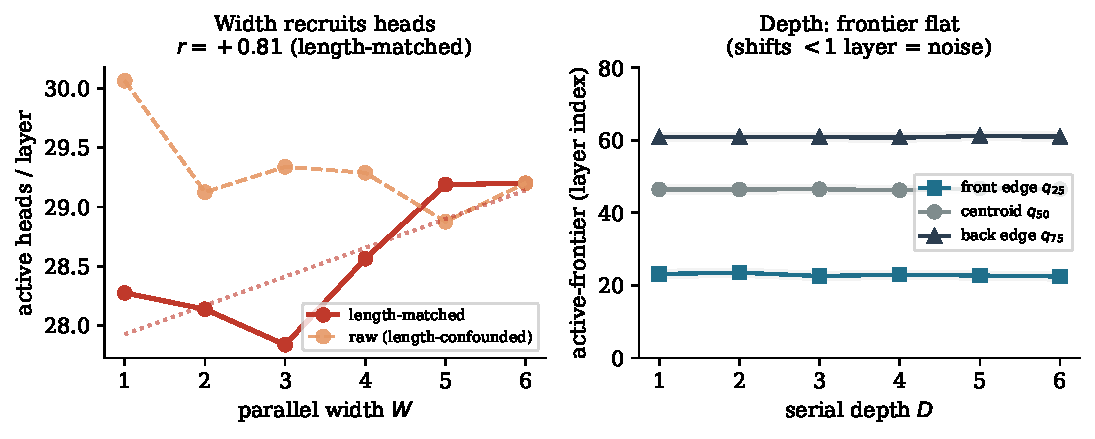
\includegraphics[width=\linewidth]{figs/fig_axes.pdf}
\caption{The two axes on Llama-3-70B. \textbf{Left:} parallel width recruits
heads (active heads/layer vs.\ $W$, length-matched, $r{=}{+}0.81$); the raw
(non-length-matched) curve trends the opposite way---a length artifact that the
control removes. \textbf{Right:} serial depth does \emph{not} move the active
frontier: the front/centroid/back quantiles shift by $<1$ layer across
$D{=}1\ldots6$ (grey band $=\pm1$ layer), i.e.\ within noise.}
\label{fig:axes}
\end{figure}

\paragraph{The length control is necessary.}
The \emph{raw} parallel ladder shows active heads \emph{falling} with $W$---the
opposite of the prediction---but this reverses once prompt length is held
constant (Figure~\ref{fig:axes} left, dashed vs.\ solid). The raw trend is a
length artifact (a longer prompt leaves more heads below threshold at the final
token); only the length-matched ladder reveals the true width effect. We
therefore treat length matching as mandatory for the width axis.

\paragraph{The depth axis is not resolved on the 70B (a null, not a
refutation).}
Serial depth produces \emph{no} detectable frontier extension here: across
$D{=}1\ldots6$ the front-edge, centroid, and back-edge of the active region
each shift by less than one layer on an 80-layer network
(Figure~\ref{fig:axes} right)---noise. We read this as an instrument problem,
not evidence against the hypothesis. A 70B idles $\sim$half its heads
(Section~\ref{sec:scale}), so a six-step task is trivially within capacity and
barely perturbs the geometry; and without accuracy measurements we cannot
verify the model computes the pointer-chase serially at all. The depth axis
must be tested where the reserve is small---the GPT-2/Pythia models, on which
six hops is a large fraction of total depth---with per-cell accuracy and
paraphrase replicates. We state this explicitly so the confirmed width axis is
not over-read into a full dissociation.

% ======================================================================
\section{Interpretation}
% ======================================================================
The measurements support a compact two-axis account. Treat each model as
holding a reserve of dormant attention heads that it \emph{recruits} on
demand.

\emph{Vertical axis (recruitment).} Rising task demand---most cleanly,
additional reasoning steps---is paid for by activating more of this reserve,
so $\dl$ deflates monotonically. The size of the reserve, and how much of it
is mobilised, are set by model capacity: larger models hold more idle width
and mobilise more of it under load.

\emph{Horizontal axis (frontier extension).} The recruitment is not
spatially uniform. Each additional composition step pulls the active frontier
deeper into the network: early and middle layers that idle on a shallow task
are engaged on a deeper one, and the front edge of the dead zone retreats
(Section~\ref{sec:frontier}). This advance has an estimable per-hop layer
cost and appears to plateau when the model runs out of usable depth, linking
the geometry directly to the serial-depth limits of transformers
\citep{merrill2023parallelism,yang2024large,biran2024hopping}.

The two axes are coupled---more demand both deflates the landscape and
advances its frontier---and both are gated by spare capacity, which is why
they emerge in the larger models and vanish into noise in the smallest. The
deformation acts on a conserved backbone: a task-invariant sparse readout
region at the back persists at every difficulty, while the action happens in
the early-to-middle band. In short: a capacity-gated recruitment response with
a magnitude (how many heads) and a reach (how deep).

% ======================================================================
\section{Limitations}
% ======================================================================
\begin{enumerate}[leftmargin=1.4em,itemsep=2pt]
\item \textbf{Data recovered from figures.} Counts are recovered from rendered
bar charts (Section~\ref{sec:method}); they are validated to $\pm1$--$2$ heads
but are not the exact arrays. Regenerating numeric data from the pipeline is
the first roadmap item.
\item \textbf{Small models are noisy.} Pythia-70M/160M have few heads, so
their counts are quantisation-noisy and some rungs are non-monotone
(Table~\ref{tab:dc-total}); the clean trends rest on the larger models.
\item \textbf{Single threshold.} ``Dead'' is defined at $\tau=0.15$; the
robustness of the trend to $\tau$ must be demonstrated.
\item \textbf{Width and reasoning depth are not separated.} The
\texttt{deep\_chains} ladder raises reasoning depth and, incidentally, the
number of intermediate entities to hold; a width-only control is required to
attribute the vertical axis to demand and the horizontal axis to serial depth
specifically.
\item \textbf{The horizontal axis rests partly on recovered data.} The
frontier correlations are strongest and cleanest on the exact Llama-3-8B data
($r{=}{+}0.96$) but modest on individual figure-recovered models; the pooled
estimate ($r{=}{+}0.70$) and the exact check are what carry it. It should be
reproduced on exact data across the full sweep.
\item \textbf{No behavioural correlate yet.} We have not tied either axis to
task accuracy; the prediction is that both recruitment and frontier advance
track whether the model can actually perform the task, and that the frontier
plateau coincides with the accuracy collapse.
\item \textbf{Single prompt per condition.} No paraphrase variance is
reported, so surface-length confounds are not yet excluded.
\end{enumerate}

% ======================================================================
\section{Roadmap: experiments to finish the paper}\label{sec:roadmap}
% ======================================================================
The following is an ordered, concrete plan to convert these observations into
a strong submission.

\paragraph{A. Regenerate exact numeric data (removes Limitation~1).}
Add a \texttt{--dump-dead-matrix} option to the analysis pipeline that writes
the full per-$(\ell,h)$ attribution and the binary dead mask to CSV/JSON for
every (model, task), and rerun the six-model sweep. All tables in this paper
should then be regenerated from exact arrays.

\paragraph{B. Dissociate recruitment from reasoning depth (the key control).}
Add a \emph{width-control} suite that raises parallel demand at fixed
reasoning depth---e.g.\ retrieve $k$ \emph{independent}, non-chained facts in
one prompt for $k=1\ldots6$. Prediction: dead-head count falls with $k$ (more
heads recruited) even though no additional composition step is added. This is
the experiment that establishes recruitment as a demand response rather than a
depth artefact.

\paragraph{C. Tie both axes to behaviour.}
Score every model on every rung of every ladder (exact-match accuracy on the
final entity). Test two predictions: (i) recruitment co-varies with
success---where a model cannot perform the task, recruitment stalls; and
(ii) the \emph{active frontier plateaus at the depth where accuracy
collapses}, making the frontier a read-out of the model's usable serial depth.
Report, per model, the correlation of accuracy with both dead-head count and
frontier depth $q_{25}$.

\paragraph{C$'$. Confirm the horizontal axis on exact data across the sweep.}
The frontier effect is clean on exact Llama-3-8B attribution but rests on
pooled/recovered estimates for the GPT-2/Pythia models. Recompute $q_{25}$,
the centroid, and early-layer dead counts from the exact masks of item~A for
all models and rungs, and report per-model $r(\text{hops},q_{25})$ with
confidence intervals. This converts the headline two-axis result from
``suggestive across models, exact on one'' to ``exact across all.''

\paragraph{D. Threshold robustness.}
Recompute all results for $\tau\in\{0.05,0.10,0.15,0.20\}$ and show the
recruitment trend (sign and approximate magnitude) is invariant. Include as a
supplementary figure.

\paragraph{E. Paraphrase and statistical rigour.}
Generate $\geq5$ surface paraphrases per condition (renamed entities, reordered
clauses, matched token length) and report means with confidence intervals and a
per-model Spearman $\rho$(demand, dead-count). This rules out length/surface
confounds and quantifies significance.

\paragraph{F. Extend to instruction-tuned and larger models.}
Repeat the cleanest ladder (\texttt{deep\_chains}, width-control) on at least
one modern model family (e.g.\ a Llama-3 or Pythia-1.4B/2.8B series) to test
whether the scale-dilation trend continues; restoring per-head attribution on
the large-model path is a prerequisite.

\paragraph{G. Head-identity analysis (optional, strengthens mechanism).}
Track \emph{which} heads are recruited as demand rises---are they consistent
across prompts, do early-recruited heads correspond to known functional types?
This connects the aggregate count to the circuits literature.

\paragraph{H. Two headline figures.}
(i) A small-multiples panel of $\dl$ for all six models $\times$ six rungs,
with the conserved sparse readout region shaded, so the recruitment-and-scale
story is legible at a glance. (ii) A two-axis summary: per model, total dead
(vertical) and frontier depth $q_{25}$ (horizontal) as functions of hop count,
so the coupled deformation and its scale dependence are visible together.

\paragraph{Deliverables checklist.}
exact-data regeneration (A) $\to$ width control (B) $\to$ behaviour coupling
(C) $\to$ exact two-axis confirmation (C$'$) $\to$ robustness + statistics
(D, E) $\to$ scale extension (F) $\to$ optional mechanism (G) $\to$ headline
figures (H). Items A--E and C$'$ are necessary for a credible submission;
F--H strengthen it.

% ======================================================================
\section{Conclusion}
% ======================================================================
We introduced the dead-head landscape as a graded probe of how transformers
allocate their attention machinery to a task, and established a two-axis
demand--geometry law. As task demand rises the landscape deforms in two
coupled ways: it \emph{deflates}---models monotonically engage dormant heads,
drawing on a reserve whose size scales with capacity (vertical
recruitment)---and its \emph{active frontier advances}---each additional
reasoning step pulls computation deeper into the network at an estimable
per-hop layer cost (horizontal extension). Both effects are gated by spare
capacity, emerging in larger models and washing out in the smallest. The full
dataset and a concrete experimental roadmap are provided so the result can be
completed and validated.

% ======================================================================
\appendix
\section{Complete dataset}\label{app:data}
% ======================================================================
All $84$ measurements recovered from \texttt{abdulla\_results/}. ``Frac'' is
dead heads over total heads; ``$q_{25}$'' is the front-edge depth (horizontal
axis: normalised depth at which the first quarter of dead mass accumulates);
``Centroid'' is the dead-mass centre in fractional depth ($0=$ first layer,
$1=$ last); ``Front'' is the fraction of dead mass in the first half of the
network.

\subsection{\texttt{complexity\_gradient} suite (48 measurements)}
\small
\begin{longtable}{lllrrrrr}
\toprule
Model & Geom (L$\times$H) & Task & Dead & Frac & $q_{25}$ & Centroid & Front \\
\midrule
\endfirsthead
\toprule
Model & Geom (L$\times$H) & Task & Dead & Frac & $q_{25}$ & Centroid & Front \\
\midrule
\endhead
\bottomrule
\endfoot
\input{app_cg_rows.tex}
\end{longtable}

\subsection{\texttt{deep\_chains} suite (36 measurements)}
\small
\begin{longtable}{lllrrrrr}
\toprule
Model & Geom (L$\times$H) & Task & Dead & Frac & $q_{25}$ & Centroid & Front \\
\midrule
\endfirsthead
\toprule
Model & Geom (L$\times$H) & Task & Dead & Frac & $q_{25}$ & Centroid & Front \\
\midrule
\endhead
\bottomrule
\endfoot
\input{app_dc_rows.tex}
\end{longtable}

% ======================================================================
\begin{thebibliography}{99}
\small

\bibitem[Belrose et al.(2023)]{belrose2023eliciting}
N.~Belrose et al.
\newblock Eliciting latent predictions from transformers with the tuned lens.
\newblock \emph{arXiv:2303.08112}, 2023.

\bibitem[Biran et al.(2024)]{biran2024hopping}
E.~Biran et al.
\newblock Hopping too late: Exploring the limitations of latent multi-hop
reasoning in large language models.
\newblock \emph{EMNLP}, 2024.

\bibitem[Conmy et al.(2023)]{conmy2023towards}
A.~Conmy et al.
\newblock Towards automated circuit discovery for mechanistic interpretability.
\newblock \emph{NeurIPS}, 2023.

\bibitem[Dehghani et al.(2019)]{dehghani2019universal}
M.~Dehghani et al.
\newblock Universal transformers.
\newblock \emph{ICLR}, 2019.

\bibitem[Elbayad et al.(2020)]{elbayad2020depth}
M.~Elbayad et al.
\newblock Depth-adaptive transformer.
\newblock \emph{ICLR}, 2020.

\bibitem[Elhage et al.(2021)]{elhage2021mathematical}
N.~Elhage et al.
\newblock A mathematical framework for transformer circuits.
\newblock \emph{Anthropic}, 2021.

\bibitem[Fan et al.(2020)]{fan2020reducing}
A.~Fan, E.~Grave, A.~Joulin.
\newblock Reducing transformer depth on demand with structured dropout.
\newblock \emph{ICLR}, 2020.

\bibitem[Feng et al.(2023)]{feng2023towards}
G.~Feng et al.
\newblock Towards revealing the mystery behind chain of thought: A theoretical
perspective.
\newblock \emph{NeurIPS}, 2023.

\bibitem[Ferrando \& Voita(2024)]{ferrando2024information}
J.~Ferrando, E.~Voita.
\newblock Information flow routes: Automatically interpreting language models at
scale.
\newblock \emph{EMNLP}, 2024.

\bibitem[Geva et al.(2023)]{geva2023dissecting}
M.~Geva et al.
\newblock Dissecting recall of factual associations in auto-regressive language
models.
\newblock \emph{EMNLP}, 2023.

\bibitem[Graves(2016)]{graves2016adaptive}
A.~Graves.
\newblock Adaptive computation time for recurrent neural networks.
\newblock \emph{arXiv:1603.08983}, 2016.

\bibitem[Gromov et al.(2024)]{gromov2024unreasonable}
A.~Gromov et al.
\newblock The unreasonable ineffectiveness of the deeper layers.
\newblock \emph{arXiv:2403.17887}, 2024.

\bibitem[Lad et al.(2024)]{lad2024remarkable}
V.~Lad, W.~Gurnee, M.~Tegmark.
\newblock The remarkable robustness of LLMs: Stages of inference.
\newblock \emph{arXiv:2406.19384}, 2024.

\bibitem[Li et al.(2024)]{li2024chain}
Z.~Li et al.
\newblock Chain of thought empowers transformers to solve inherently serial
problems.
\newblock \emph{ICLR}, 2024.

\bibitem[Men et al.(2024)]{men2024shortgpt}
X.~Men et al.
\newblock ShortGPT: Layers in large language models are more redundant than you
expect.
\newblock \emph{arXiv:2403.03853}, 2024.

\bibitem[Meng et al.(2022)]{meng2022locating}
K.~Meng et al.
\newblock Locating and editing factual associations in GPT.
\newblock \emph{NeurIPS}, 2022.

\bibitem[Merrill \& Sabharwal(2023)]{merrill2023parallelism}
W.~Merrill, A.~Sabharwal.
\newblock The parallelism tradeoff: Limitations of log-precision transformers.
\newblock \emph{TACL}, 2023.

\bibitem[Michel et al.(2019)]{michel2019sixteen}
P.~Michel, O.~Levy, G.~Neubig.
\newblock Are sixteen heads really better than one?
\newblock \emph{NeurIPS}, 2019.

\bibitem[Nanda(2023)]{nanda2023attribution}
N.~Nanda.
\newblock Attribution patching: Activation patching at industrial scale.
\newblock Technical report, 2023.

\bibitem[nostalgebraist(2020)]{nostalgebraist2020logitlens}
nostalgebraist.
\newblock Interpreting GPT: The logit lens.
\newblock \emph{LessWrong}, 2020.

\bibitem[Raposo et al.(2024)]{raposo2024mixture}
D.~Raposo et al.
\newblock Mixture-of-depths: Dynamically allocating compute in
transformer-based language models.
\newblock \emph{arXiv:2404.02258}, 2024.

\bibitem[Sajjad et al.(2023)]{sajjad2023effect}
H.~Sajjad et al.
\newblock On the effect of dropping layers of pre-trained transformer models.
\newblock \emph{Computer Speech \& Language}, 2023.

\bibitem[Schuster et al.(2022)]{schuster2022confident}
T.~Schuster et al.
\newblock Confident adaptive language modeling.
\newblock \emph{NeurIPS}, 2022.

\bibitem[Voita et al.(2019)]{voita2019analyzing}
E.~Voita et al.
\newblock Analyzing multi-head self-attention: Specialized heads do the heavy
lifting, the rest can be pruned.
\newblock \emph{ACL}, 2019.

\bibitem[Wang et al.(2022)]{wang2022interpretability}
K.~Wang et al.
\newblock Interpretability in the wild: A circuit for indirect object
identification in GPT-2 small.
\newblock \emph{ICLR}, 2023 (arXiv 2022).

\bibitem[Xin et al.(2020)]{xin2020deebert}
J.~Xin et al.
\newblock DeeBERT: Dynamic early exiting for accelerating BERT inference.
\newblock \emph{ACL}, 2020.

\bibitem[Yang et al.(2024)]{yang2024large}
S.~Yang et al.
\newblock Do large language models latently perform multi-hop reasoning?
\newblock \emph{ACL}, 2024.

\end{thebibliography}

\end{document}
